% Data visualization with pgfplots -- demonstration project
% All data are computed or synthetic (see generate_data.ps1), none are measured.
% Compile with: latexmk -pdf main.tex
\documentclass[a4paper,10pt]{article}
\usepackage[a4paper,landscape,margin=1.4cm,top=1.5cm,bottom=1.3cm]{geometry}
\usepackage[T1]{fontenc}
\usepackage[utf8]{inputenc}
\usepackage{amsmath,amssymb}
\usepackage{newpxtext,newpxmath}
\usepackage{microtype}
\usepackage{xcolor}
\usepackage{tikz}
\usepackage{pgfplots}
\usepgfplotslibrary{groupplots}
\pgfplotsset{compat=1.18}

\definecolor{wine}{HTML}{7F1D1D}
\definecolor{ink}{HTML}{1C1917}
\definecolor{sea}{HTML}{1D4E89}
\definecolor{moss}{HTML}{2F6B3A}
\definecolor{ochre}{HTML}{B7791F}
\definecolor{paper}{HTML}{FBF7EE}
\definecolor{sand}{HTML}{F3ECDA}
\definecolor{line}{HTML}{DDD2B8}

\pagecolor{paper}
\color{ink}
\pagestyle{empty}
\setlength{\parindent}{0pt}

\newcommand{\panel}[3]{% title, height, content
  \begin{minipage}[t]{0.322\textwidth}
    {\scshape\color{wine}\small #1}\par\vspace{2pt}
    {\color{line}\hrule height 0.6pt}\vspace{6pt}
    \begin{minipage}[c][#2][c]{\linewidth}\centering #3\end{minipage}
  \end{minipage}%
}

\pgfplotsset{
  every axis/.append style={
    width=\linewidth, height=5.5cm,
    font=\footnotesize, tick label style={font=\scriptsize},
    label style={font=\footnotesize},
    axis line style={ink!70}, tick style={ink!70},
    grid=major, grid style={line!70, line width=0.3pt},
    legend style={font=\scriptsize, fill=paper, fill opacity=0.9, draw=line, text opacity=1, cells={anchor=west}},
  },
  every axis plot/.append style={thick},
}

\begin{document}

\begin{minipage}[b]{0.7\textwidth}
  {\Huge\bfseries Data visualization with pgfplots}\\[2pt]
  {\large\itshape Six publication-quality plots, drawn from CSV files directly inside \LaTeX.}
\end{minipage}\hfill
\begin{minipage}[b]{0.28\textwidth}\raggedleft\small
  Demonstration project\\
  pgfplots \textperiodcentered{} CSV tables \textperiodcentered{} log scales
\end{minipage}

\vspace{4pt}{\color{wine}\hrule height 1.2pt}\vspace{10pt}

\panel{1 \quad Convergence of one-step methods}{6.9cm}{%
\begin{tikzpicture}
\begin{loglogaxis}[
  xlabel={step size $h$}, ylabel={error at $t=1$},
  xmin=3e-3, xmax=0.4, ymin=1e-14, ymax=1,
  legend pos=south east,
  xtick={0.004,0.0156,0.0625,0.25}, xticklabels={$2^{-8}$,$2^{-6}$,$2^{-4}$,$2^{-2}$},
  ytick={1e-12,1e-9,1e-6,1e-3,1},
]
  \addplot[wine,mark=square*,mark size=1.6pt] table[col sep=comma,x=h,y=euler] {convergence.csv};
  \addlegendentry{Euler, order 1}
  \addplot[sea,mark=*,mark size=1.6pt] table[col sep=comma,x=h,y=heun] {convergence.csv};
  \addlegendentry{Heun, order 2}
  \addplot[moss,mark=triangle*,mark size=2pt] table[col sep=comma,x=h,y=rk4] {convergence.csv};
  \addlegendentry{RK4, order 4}
\end{loglogaxis}
\end{tikzpicture}}
\hfill
\panel{2 \quad Predator--prey populations}{6.9cm}{%
\begin{tikzpicture}
\begin{axis}[
  xlabel={time $t$}, ylabel={population},
  xmin=0, xmax=30, ymin=0,
  legend pos=north east,
]
  \addplot[sea,no marks] table[col sep=comma,x=t,y=prey] {predator_prey.csv};
  \addlegendentry{prey}
  \addplot[wine,no marks] table[col sep=comma,x=t,y=predator] {predator_prey.csv};
  \addlegendentry{predator}
\end{axis}
\end{tikzpicture}}
\hfill
\panel{3 \quad Phase portrait}{6.9cm}{%
\begin{tikzpicture}
\begin{axis}[
  xlabel={prey}, ylabel={predator},
  xmin=0, ymin=0,
  legend pos=north east,
]
  \addplot[ochre,no marks] table[col sep=comma,x=prey,y=predator] {predator_prey.csv};
  \addlegendentry{orbit}
  \addplot[only marks,mark=*,mark size=2.2pt,wine] coordinates {(20,10)};
  \addlegendentry{equilibrium}
  \addplot[only marks,mark=o,mark size=2.2pt,ink] coordinates {(10,5)};
  \addlegendentry{start}
\end{axis}
\end{tikzpicture}}

\vspace{12pt}

\panel{4 \quad Cost to reach error $\le 10^{-6}$}{6.9cm}{%
\begin{tikzpicture}
\begin{axis}[
  ybar, bar width=18pt, ymode=log, log origin=infty,
  symbolic x coords={Euler,Heun,RK4}, xtick=data,
  ylabel={function evaluations}, ymin=10, ymax=1e8,
  enlarge x limits=0.3,
  point meta=explicit,
  nodes near coords={\pgfmathprintnumber[sci,precision=1]{\pgfplotspointmeta}},
  nodes near coords style={font=\scriptsize,/pgf/number format/sci generic={mantissa sep=\times,exponent={10^{##1}}}},
  ytick={10,1e2,1e4,1e6,1e8},
]
  \addplot[fill=ochre!70,draw=ochre!90!ink] table[col sep=comma,x=method,y=evals,meta=evals] {cost.csv};
\end{axis}
\end{tikzpicture}}
\hfill
\panel{5 \quad Surface $z = x\,e^{-x^2-y^2}$}{6.9cm}{%
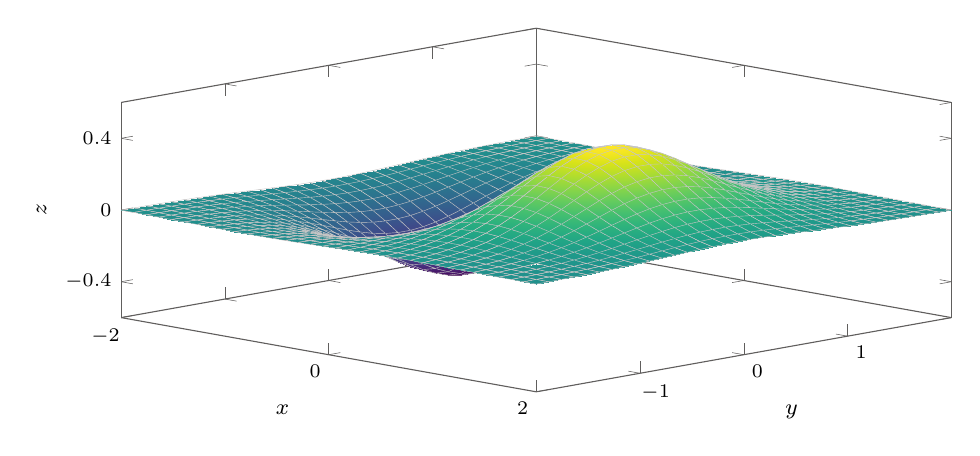
\begin{tikzpicture}
\begin{axis}[
  view={45}{26}, grid=none, height=6.2cm,
  xlabel={$x$}, ylabel={$y$}, zlabel={$z$},
  colormap/viridis, colorbar=false,
  xtick={-2,0,2}, ytick={-1,0,1}, ztick={-0.4,0,0.4},
  zmin=-0.6, zmax=0.6, z buffer=sort,
]
  \addplot3[surf,shader=faceted interp,faceted color=ink!25,domain=-2:2,y domain=-2:2,samples=34,samples y=34,line width=0.15pt] {x*exp(-x^2-y^2)};
\end{axis}
\end{tikzpicture}}
\hfill
\panel{6 \quad Histogram of 2\,000 samples}{6.9cm}{%
\begin{tikzpicture}
\begin{axis}[
  xlabel={value}, ylabel={density},
  xmin=-4, xmax=4, ymin=0, ymax=0.5,
  legend pos=north east,
]
  \addplot[ybar interval,fill=sea!35,draw=sea!80,forget plot,thin]
    table[col sep=comma,x=x,y=density] {histogram.csv};
  \addplot[wine,no marks,domain=-4:4,samples=80] {exp(-x^2/2)/sqrt(2*pi)};
  \addlegendentry{$\mathcal{N}(0,1)$}
\end{axis}
\end{tikzpicture}}

\vfill
{\color{line}\hrule height 0.6pt}\vspace{4pt}
{\footnotesize\color{ink!70} Source: \texttt{main.tex} + CSV files \textperiodcentered{} data are computed or synthetic (\texttt{generate\_data.ps1}) \hfill N'sol\'e Samson Yamontche \textperiodcentered{} \LaTeX{} \& pgfplots}

\end{document}
